%%%%%%%%%%%%%%%%%%%%%%%%%%%%%%%%%%%%%%%%%%%%%%%%%%%%
%%											  	 %%
%% Author : Andreas Apostolatos               	 %%
%%											  	 %%
%% e-mail : andreas.apostolatos@tum.de		   	 %%
%%											  	 %%
%% 07_Results.tex					  	   	 	 %%
%%											  	 %%
%%%%%%%%%%%%%%%%%%%%%%%%%%%%%%%%%%%%%%%%%%%%%%%%%%%%

\section{Results}

\subsection{Displacement sensitivity}

Since the displacement sensitivity has a local meaning, a node has to be selected within the mesh, where the analysis is request to be performed. In this case, node 144 - circled in red in figure \ref{cantileverBeam:nodeOfInterest} below - has been chosen. It is situated in the middle of the free end of the cantilever beam. \\
\begin{figure}[ht]
\centering
  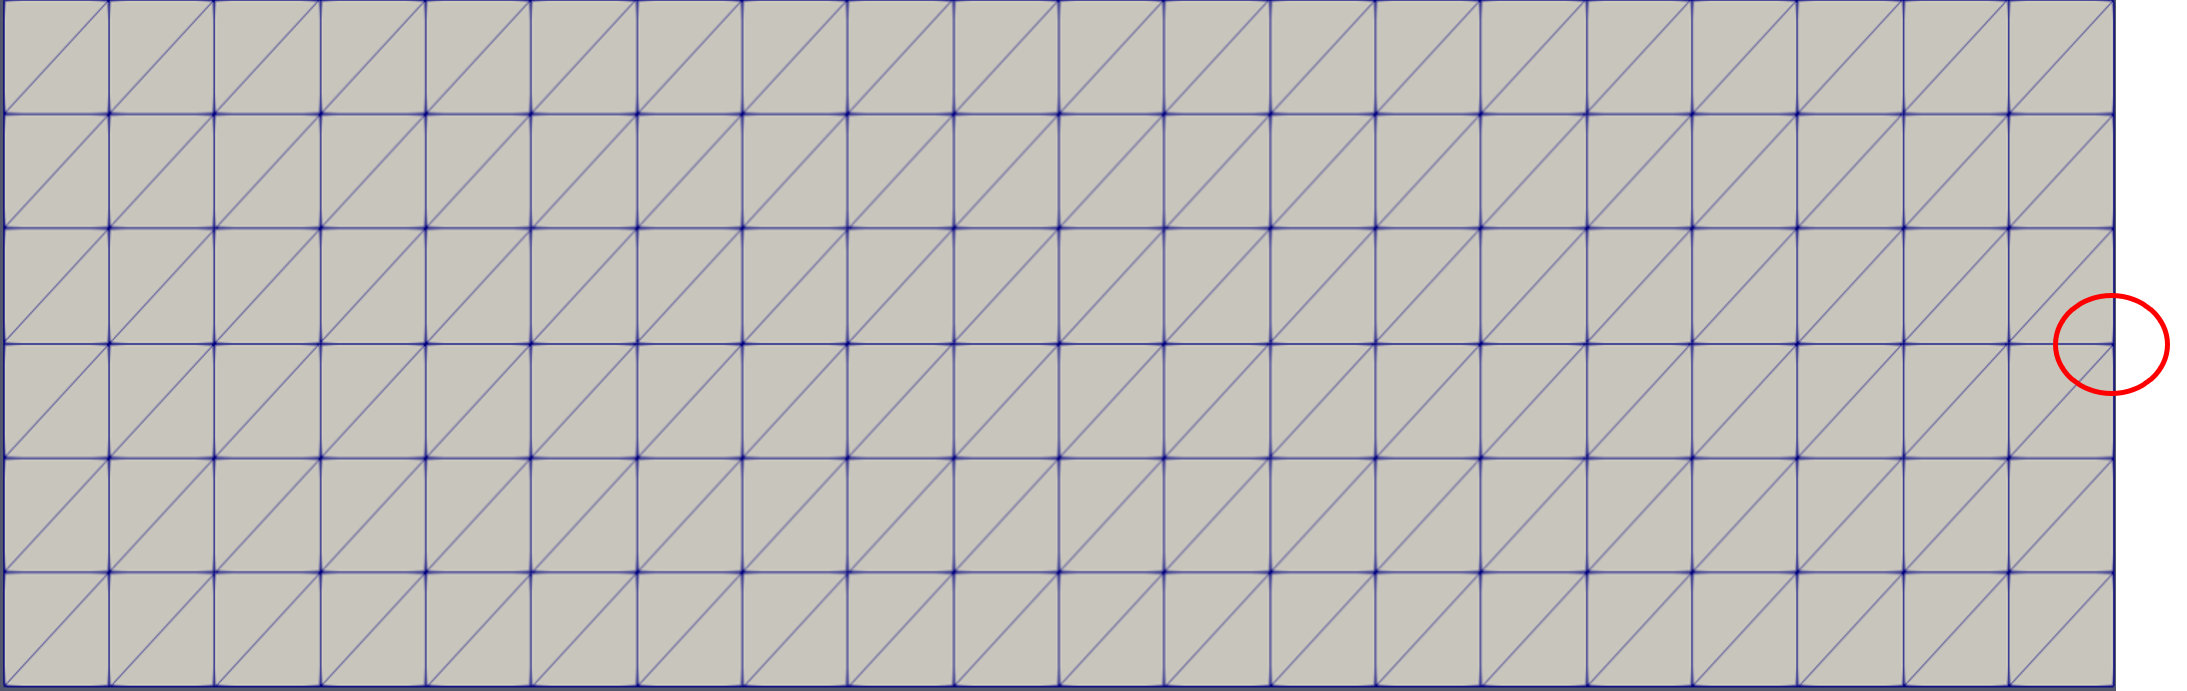
\includegraphics[width=100mm]{images/meshNodeOfInterest.png}
  \caption{Node 144}
  \label{cantileverBeam:nodeOfInterest}
\end{figure}\\
Since the perturbation is performed separately in $x$ and $y$ direction, two different plots are shown below, in order to clearly represent which influence is due to which perturbation. \\
\begin{figure}[ht]
\centering
\begin{minipage}{.5\textwidth}
  \centering
  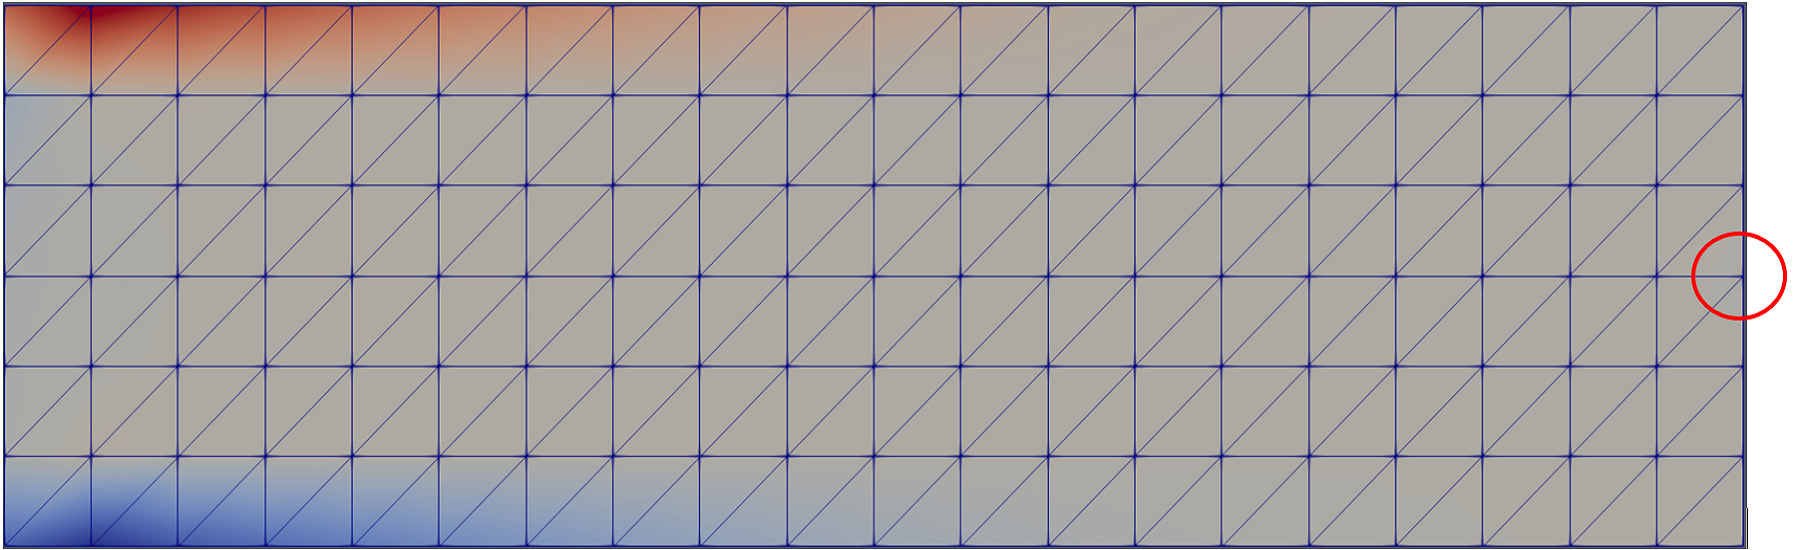
\includegraphics[width=1.0\linewidth]{images/sensitivityanalysisY.png}
  \captionof{figure}{displacement sensitivity, y-perturbation}
  \label{fig:yDispSens}
\end{minipage}%
\begin{minipage}{.5\textwidth}
  \centering
  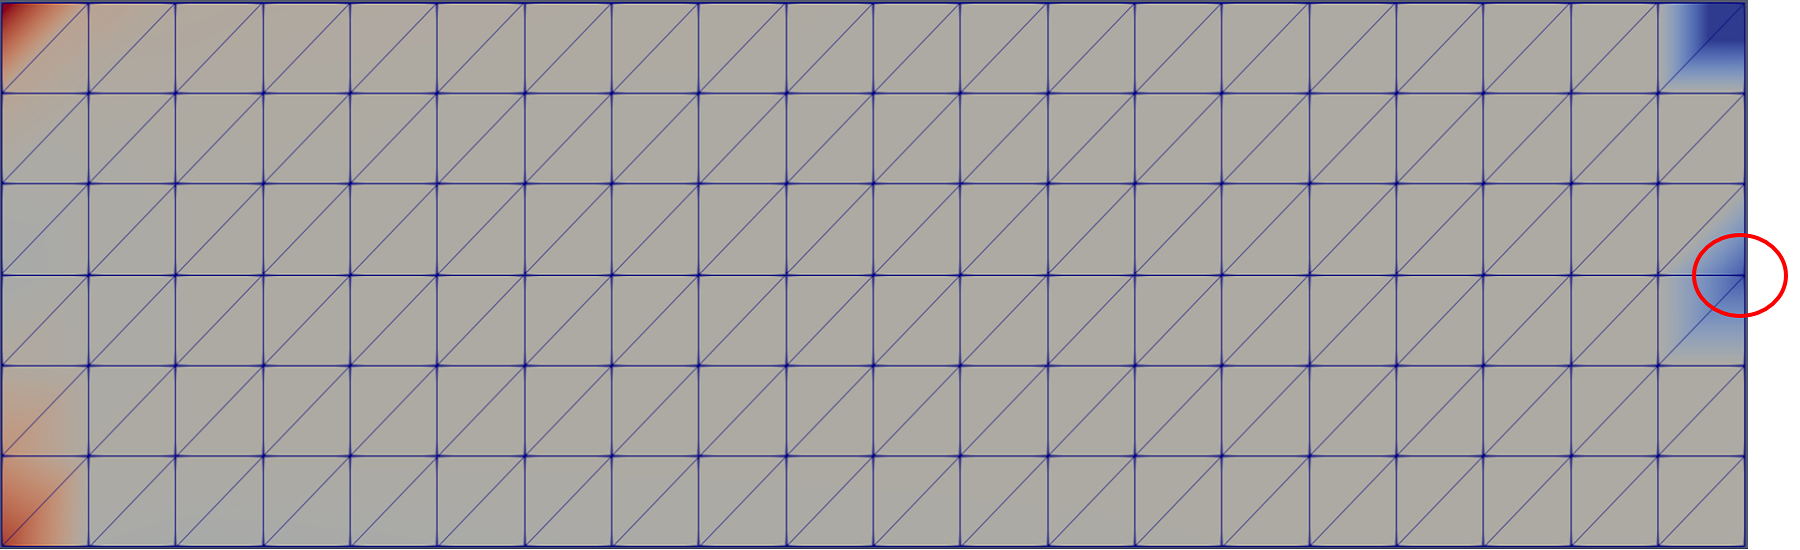
\includegraphics[width=1.0\linewidth]{images/sensitivityanalysisX.png}
  \captionof{figure}{displacement sensitivity, x-perturbation}
  \label{fig:xDispSens}
\end{minipage}
\end{figure}\\
With these plots, a first interpretation of the analysis can be done. Intensely colored blue and red areas represent parts of the structure where a displacement of that area affects the most the displacement of node 144. \\[6pt]
Figure \ref{fig:yDispSens}, which represents the sensitivity of node 144 with respect to a perturbation of all nodes in the upward $y$-direction, is probably the more intuitive to interpret. The nodes in the upper left portion of the beam are colored red. Displacing these nodes in the upward direction effectively increases the cross sectional area of the beam. Given that this is a cantilever beam, the cross sectional area at the clamped end has the largest influence on the displacement at the free end. Therefore, displacing the upper left nodes upward increases the stiffness of the beam and reduces the displacement of node 144. Accordingly, the nodes at the bottom left of the beam reduce the cross sectional area, thereby increasing the displacement of node 144. Hence, they are colored blue.\\[6pt]
Figure \ref{fig:xDispSens} represents the sensitivity of node 144 with respect to a perturbation of all nodes in the positive $x$ (right-ward) direction. Based on the plot, displacement of the nodes in the upper left and bottom left results in lower displacement of node 144. Modifying the length of the upper surface of the beam influences the total loading. Displacing the upper left node to the right effectively reduces the length of the upper surface, thereby reducing the loading. This reduces the displacement at node 144. Displacing the upper right node to the right has the opposite effect.\\[6pt]
Further comments will be provided in the optimization section, \ref{section:optimization}.

\subsection{Strain energy sensitivity} \label{section:strainSens}
In contrast to the displacement sensitivity, the strain energy sensitivity is inherently a global value. It represents the energy of a system undergoing deformation. Equation \ref{eqn:strainenergy} from \cite{wiki:strainEnergy} below describes strain energy for a linear elastic material.\\
\begin{equation} \label{eqn:strainenergy}
U = \frac{1}{2}V\sigma\epsilon
\end{equation}\\
Where $V$ represents the volume of the structure, $\sigma$ represents stress, and $\epsilon$ represents strain. Since the energy of the structure is global, a node does not need to be chosen; the analysis is performed on the entire structure. Figure \ref{fig:ystrainDispSens} and Figure \ref{fig:xstrainDispSens} below illustrate the effect on the strain energy of perturbing all nodes in the y-direction and all nodes in the x-direction, respectively. \\
\begin{figure}[ht]
\centering
\begin{minipage}{.5\textwidth}
  \centering
  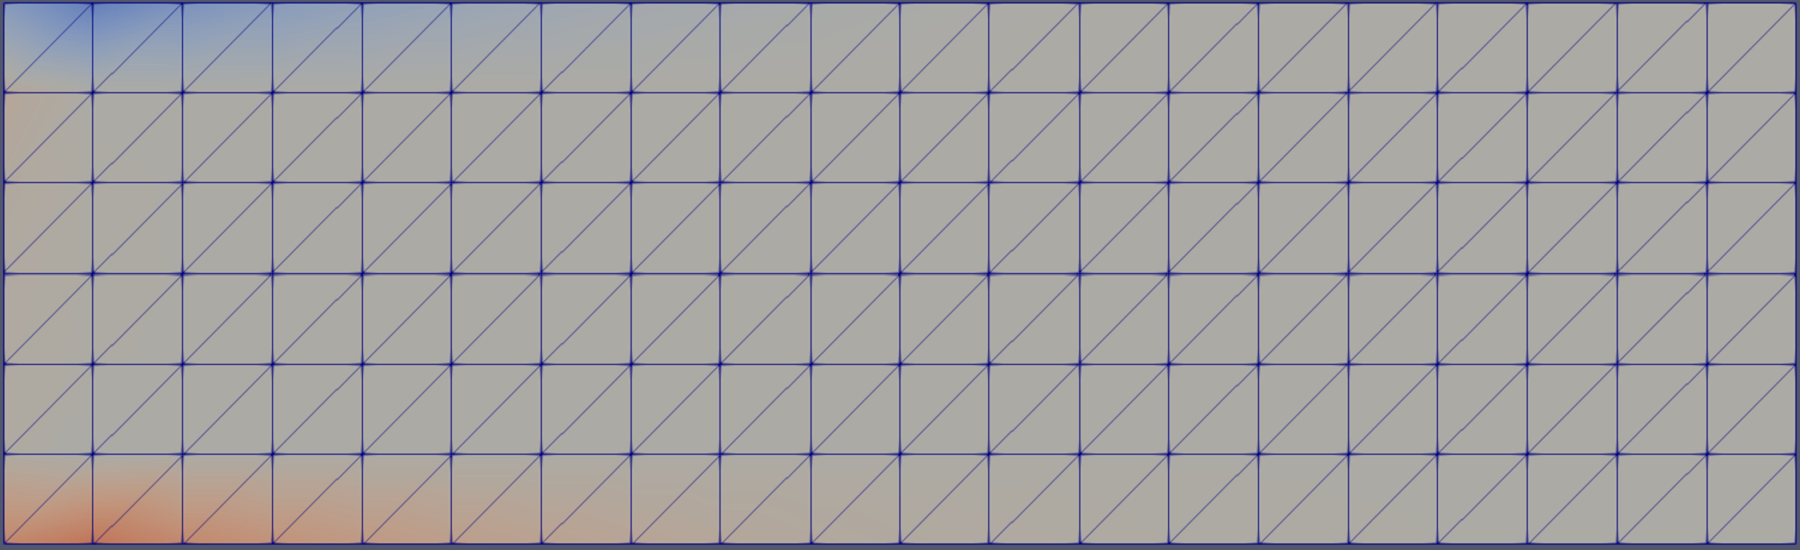
\includegraphics[width=0.95\linewidth]{images/strainsensitivityanalysisY.png}
  \captionof{figure}{strain energy sensitivity, y-perturbation}
  \label{fig:ystrainDispSens}
\end{minipage}%
\begin{minipage}{.5\textwidth}
  \centering
  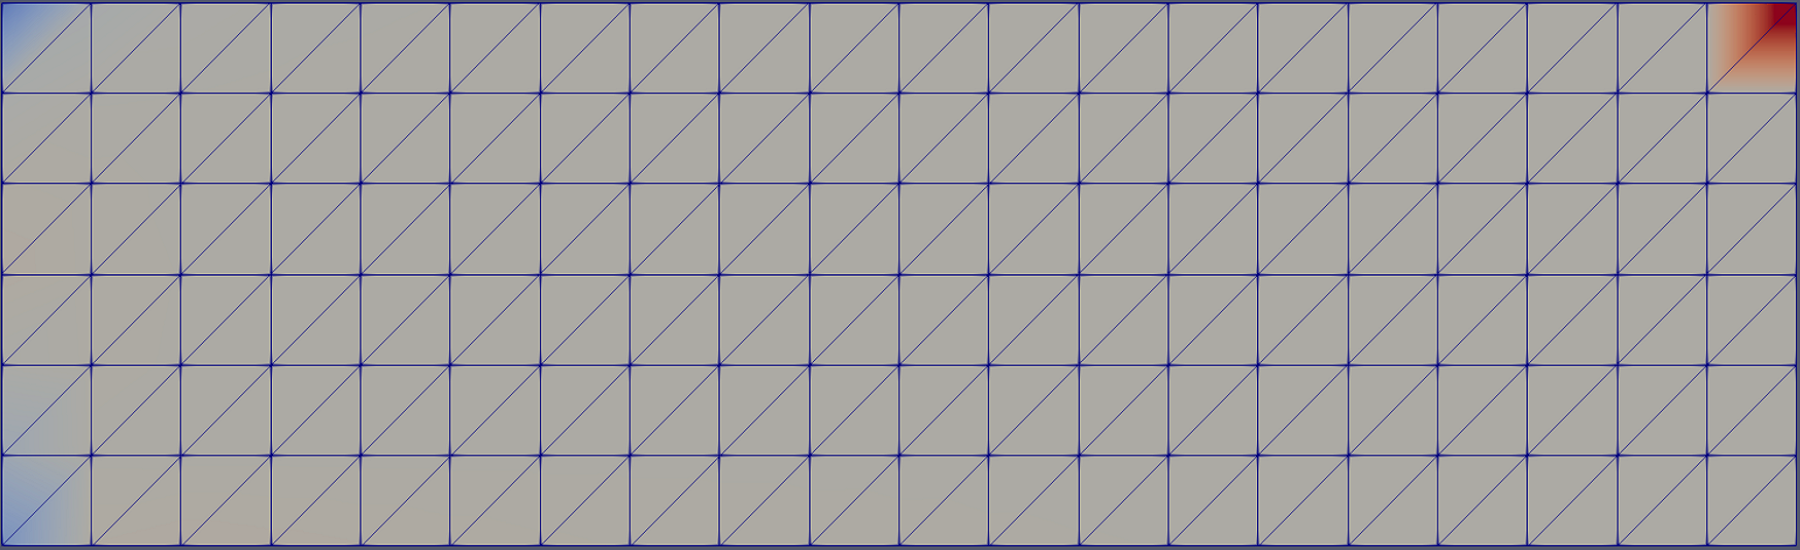
\includegraphics[width=0.95\linewidth]{images/strainsensitivityanalysisX.png}
  \captionof{figure}{strain energy sensitivity, x-perturbation}
  \label{fig:xstrainDispSens}
\end{minipage}
\end{figure}\\
In Figure \ref{fig:ystrainDispSens} above, one could make interpretations similar to those of Figure \ref{fig:yDispSens} in the previous section. In this case, the strain energy sensitivity is a function of volume, stress, and strain. The y-perturbation of nodes in the upper left and bottom right of the beam have the largest impact on the overall strain of the structure, which influences the strain energy the most. These results are very similar to those illustrated in Figure \ref{fig:yDispSens} because both simulations involve strain, which is related to displacement.\\[6pt]
Thus, it follows that the results of Figure \ref{fig:xstrainDispSens} mirror those of Figure \ref{fig:xDispSens} since the x-perturbation of the nodes along the top surface will influence the loading, which affects the overall strain energy.

\subsection{Optimization} \label{section:optimization}
Sensitivity analysis allows one to understand which parts of the structure affect most, for example, the strain energy of the structure itself. Then, how can this approach be used for optimizing the structure? \\[6pt]
For the sake of consistency, consider again the cantilever beam example. An optimization exercise may involve finding a geometry which minimizes the strain energy of the structure.\\[6pt]
As illustrated by the sensitivity analysis, it is possible to identify the areas which affect the strain energy of the system the most. So, the structure optimization is performed as follows.
\begin{enumerate}
    \item A sensitivity analysis is performed for a specific objective function, based on user selection in GiD. If applicable, the user can select one or more node(s) or element(s)
    \item The nodal coordinates in x- and y-directions are updated by adding a particular factor found in equation \ref{eqn:nodalAdjustment} below
    \item Repeat steps 1. and 2. until desired number of iterations is reached
\end{enumerate}

\begin{equation} \label{eqn:nodalAdjustment}
    \textbf{x}_{new} = \textbf{x} + \textbf{nodalSensitivity} \cdot perturbation \cdot scalingFactor 
\end{equation}\\
As explained above, the sensitivity analysis forms the heart of the optimization algorithm. It essentially assigns a value to each node representing its effect on the objective function. Then, for each node, this sensitivity value is multiplied by the perturbation size to transform this value into a distance. Next, it is multiplied by a scaling factor to help avoid unstable behavior. Finally, it is added to the "old" nodal coordinate to form the new nodal coordinate. These steps are repeated until the maximum number of iterations, $n$, is reached. The final result is the optimized structure, which has a different shape than the starting one, and whose shape minimizes - in this case - the strain energy. \\[6pt]
Based on the results discussed in section \ref{section:strainSens}, the most sensitive areas of the structure are the upper right, upper left, and bottom left corners. Therefore, those are the areas targeted by the optimization algorithm. See Figures \ref{cantileverBeam:BCs2} and \ref{cantileverBeam:BCs2} below.\\
\begin{figure}[ht]
\centering
\begin{minipage}{.5\textwidth}
  \centering
  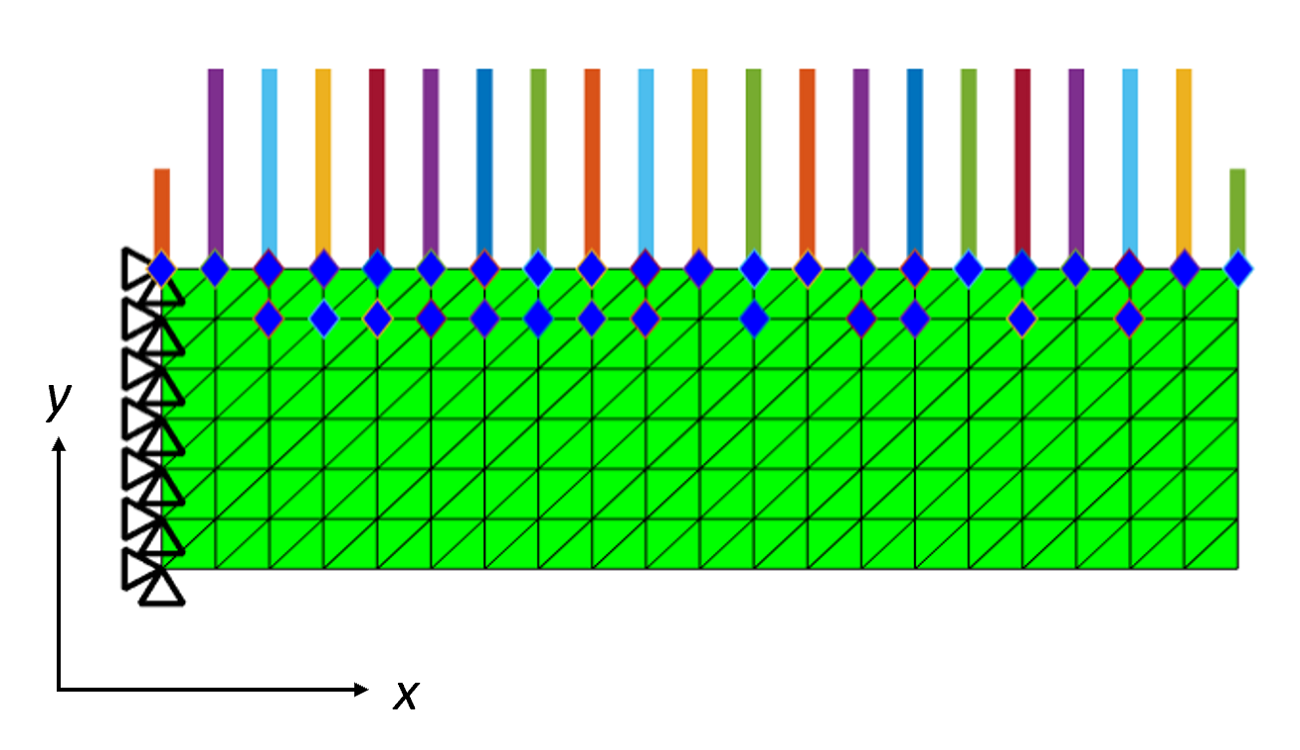
\includegraphics[width=1.0\linewidth]{images/cantileverBeamBCs.png}
  \captionof{figure}{cantilever beam, original geometry}
  \label{cantileverBeam:BCs2}
\end{minipage}%
\begin{minipage}{.5\textwidth}
  \centering
  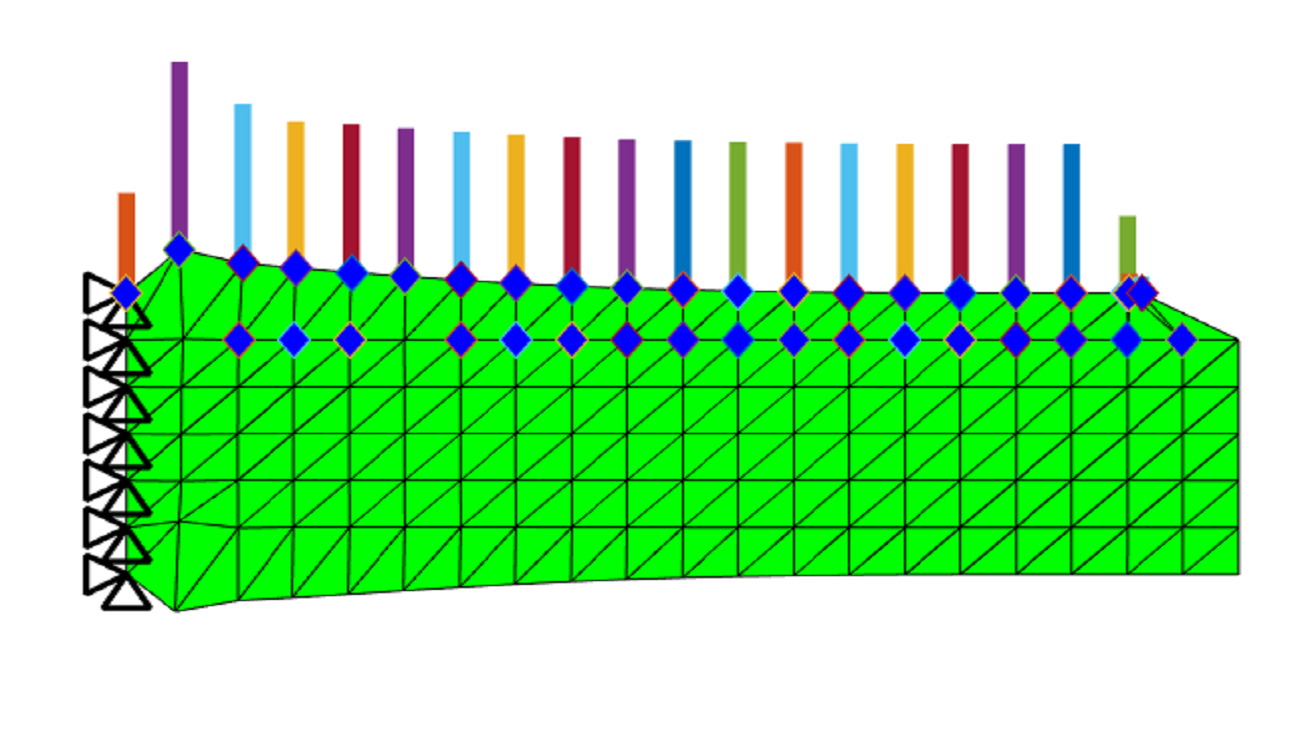
\includegraphics[width=1.0\linewidth]{images/cantileverBeamOptimized.png}
  \captionof{figure}{cantilever beam, optimized geometry}
  \label{fig:optimizedGeometry}
\end{minipage}
\end{figure}
After 10 iterations, a strain energy reduction of almost 54\% is achieved, without affecting heavily the shape of the beam. While this case considered only optimizing for strain energy, this optimization can be executed for any objective function.\\[6pt]
\begin{figure}[ht]
\centering
\begin{minipage}{.5\textwidth}
  \centering
  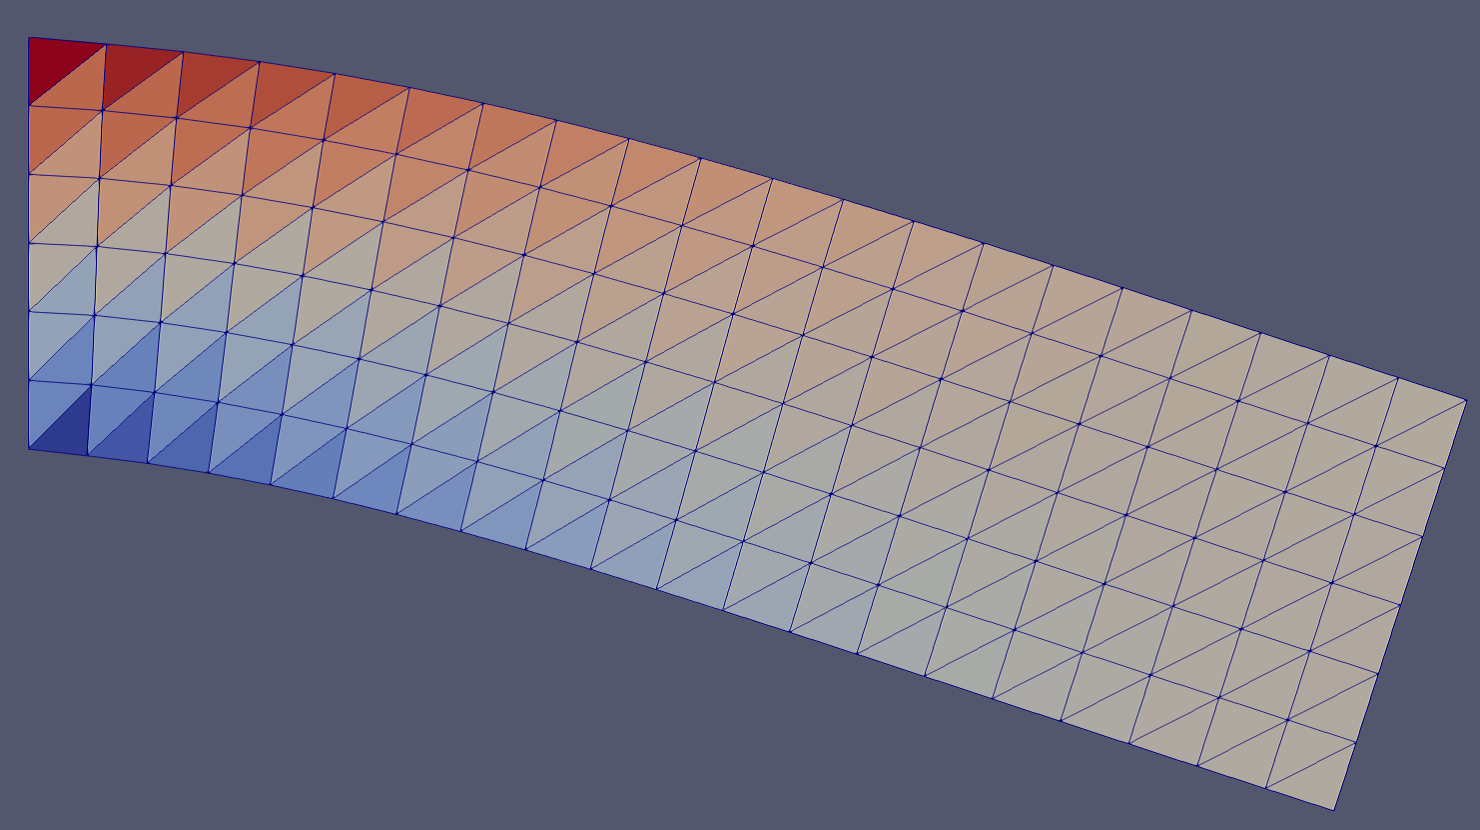
\includegraphics[width=0.9\linewidth]{images/strainAnalysis_original.png}
  \captionof{figure}{strain distribution, original geometry}
  \label{fig:strainAnalOrig}
\end{minipage}%
\begin{minipage}{.5\textwidth}
  \centering
  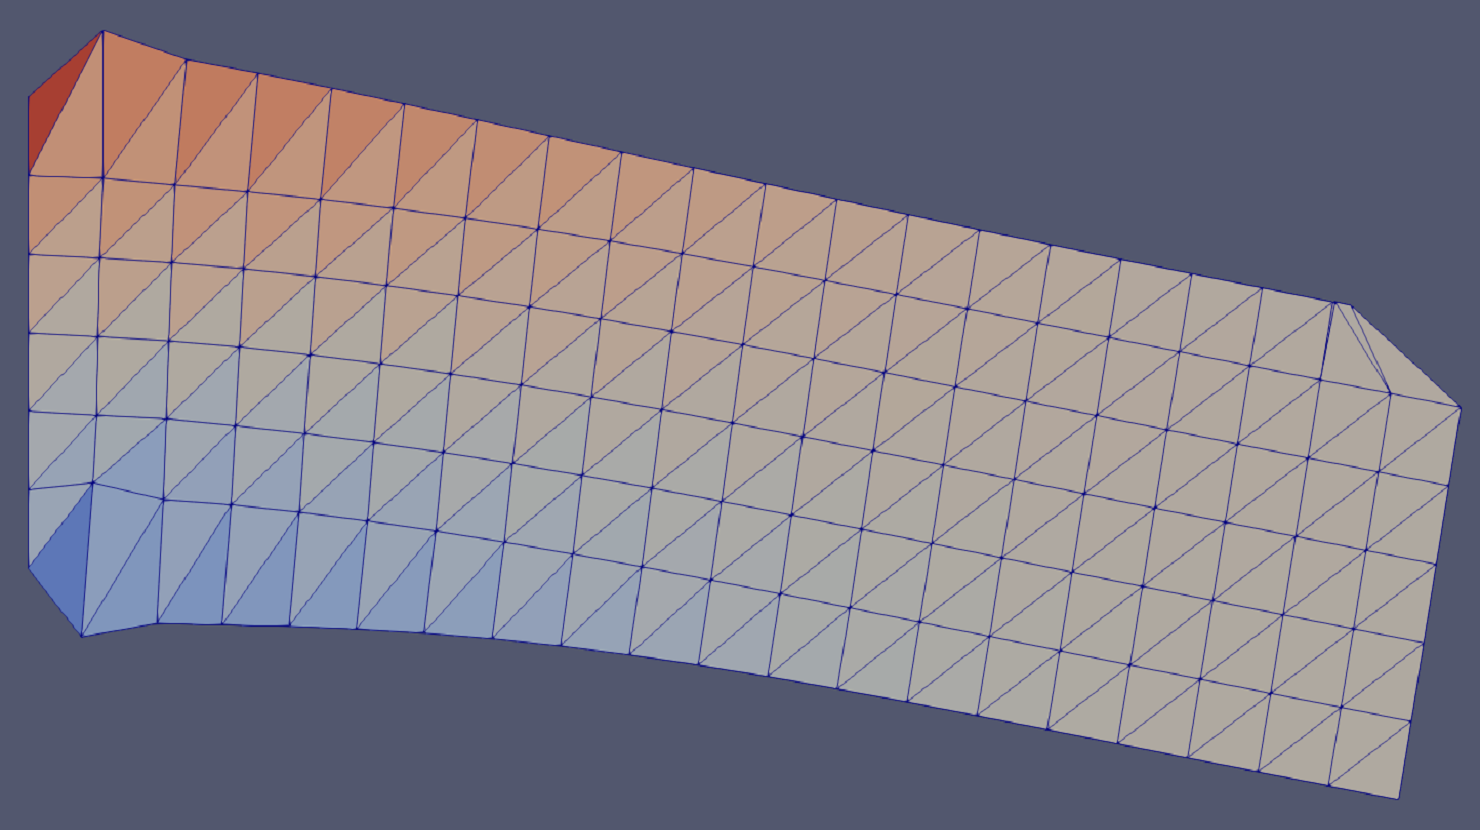
\includegraphics[width=0.9\linewidth]{images/strainAnalysis_optimized.png}
  \captionof{figure}{strain distribution, optimized geometry}
  \label{fig:strainAnalOpt}
\end{minipage}
\end{figure}
Figures \ref{fig:strainAnalOrig} and \ref{fig:strainAnalOpt} illustrate the stress distribution over the deformed cantilever beam in both the original and optimized geometry, respectively. Since the same color scale is used for both images, it is possible to qualitatively see that the strain has generally decreased from the original to the optimized geometry. This reduced strain, of course, contributes to the reduced strain energy previously mentioned.\\[6pt]
To generate this new, optimized geometry, the optimization algorithm iterated 10 times, which was predefined. This choice is primarily due to the fact that more iterations results in unstable behavior. This instability is due to the lack of an additional constraining equation. Often, multi-objective optimization is performed, whereby multiple objective functions are optimized. In this example, the algorithm would theoretically keep increasing the cross sectional area at the base, if it were not for the iteration limit. Of course, this is not realistic as engineers often want to minimize weight, volume, cost, etc. Therefore, a future improvement to this program would be to allow for optimizing multiple, opposing objective functions so that the algorithm can iterate until convergence is reached, rather than a maximum number of iterations.



